\documentclass[10pt]{article}

% set smaller margins
\usepackage[a4paper,margin=1in]{geometry}

% use standard math symbols
\usepackage{amssymb}

% for \text inside formulas and for \eqref
\usepackage{amsmath}

% for bibliography
\usepackage[sort,numbers]{natbib}

% enable full XeLaTeX power
\usepackage{xltxtra}

% select widely available fonts
\setmainfont{Georgia}
\setmonofont{Courier New}

% substitute another font for a few Unicode glyphs missing in the main font
\newfontfamily{\msminchofont}{MS Mincho}
\catcode`✓=\active
\protected\def ✓{{\msminchofont\char`\✓}}

% set paragraph margins
\setlength{\parindent}{0pt}
\setlength{\parskip}{6pt plus 2pt minus 1pt}

% prevent overfull lines
\setlength{\emergencystretch}{3em}

% for \includegraphics
\usepackage{graphicx}
\usepackage{grffile}

% fit images in page width
\makeatletter
\def\maxwidth{\ifdim\Gin@nat@width>\linewidth\linewidth
\else\Gin@nat@width\fi}
\makeatother
\let\Oldincludegraphics\includegraphics
\renewcommand{\includegraphics}[1]{\Oldincludegraphics[width=\maxwidth]{#1}}

% for exact placement of figures
\usepackage{float}

% for footnotes in tables
\usepackage{longtable}

% for hyperlinks
\usepackage[colorlinks,urlcolor=blue,filecolor=blue,linkcolor=black,citecolor=black]{hyperref}
\usepackage[all]{hypcap}
\urlstyle{same}

% do not number sections
\setcounter{secnumdepth}{0}


\begin{document}


\section{サンプル}

\subsection{例の数学公式集}

この公式集は問題と無関係に作成されたものであるが、答案作成にあたって利用してよい。この公式集は持ち帰ってよい。

\subsubsection{(不 等  式)}

\begin{itemize}
\item
  \(\dfrac{a+b}{2}\ge \sqrt{ab}, \quad \dfrac{a+b+c}{3}\ge \sqrt[3]{ab} \quad (a, b, c \;\mbox{は正または}\;0)\)
\item
  \((a^2+b^2+c^2)(x^2+y^2+z^2)\ge(ax+by+cz)^2\)
\end{itemize}

\subsubsection{(三 角 形)}

\begin{itemize}
\item
  \(\dfrac{a}{\sin A} = \dfrac{b}{\sin B} = \dfrac{c}{\sin C} = 2R\)
\item
  \(a^2=b^2+c^2 - 2bc \cos A\)
\item
  \(S=\dfrac12\sinA=\sqrt{s(s-a)(s-b)(s-c)}, \quad \left(s=\dfrac12(a+b+c)\right)\)
\end{itemize}

\subsection{キャプションの挿入}

\begin{figure}[htbp]
\centering
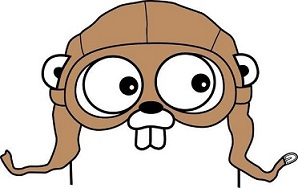
\includegraphics{img/goprogramminglanguage.jpg}
\caption{Gopher君 ((c) Go Lang Project)}
\end{figure}

\end{document}
